
\chapter{Przegląd badań - stan wiedzy}
\label{chap:theory}
    W literaturze można znaleźć prace naukowe, które badają sposoby identyfikowania aplikacji uruchamianych w środowisku superkomputerowym. Często jednak określenie typu wykonywanego programu nie jest głównych celem tych artykułów. W pracy \textit{'Using machine learning to optimize parallelism in big data applications'} autorzy próbowali poprawić estymacje planowanych zadań \cite{JobSchedulingSC}. Do identyfikacji wykorzystali metadane historyczne w celu znalezienia przeszłych uruchomień aplikacji przez danego użytkownika w ramach projektu. W zbiorze danych wykorzystywanych przez nas nie mamy takich informacji, dlatego nie możemy zastosować podobnej taktyki. 
    
    Bardziej zbliżonym artykułem był \textit{'A runtime estimation framework for ALICE'}, gdzie autorzy szukali metody poprawienia estymat długości czasu przetwarzania się aplikacji w systemie \cite{RuntimeEstimationALICE}. Chcieli oni znaleźć metody klasyfikacji typu aplikacji bez wykorzystywania metadanych. Zrobili to klasyfikując wpierw aplikacje na podstawie charakterystyk historycznych uruchomień. Nie były one niestety związane z zużyciem zasobów typu RAM oraz CPU. Do klasyfikacji został użyty algorytm drzew decyzyjnych. Uzyskał on wysoką (ok. 97\%) trafność co może być dla nas inspiracją przy wyborze algorytmów uczenia maszynowego.
    
    Potencjalnie interesującą pracą jest \textit{'Using machine learning to optimize parallelism in big data applications'}\cite{BigDataParallelism}, tutaj z kolei problemem był wybór parametrów dla przetwarzania przy użyciu technologii Spark. Autorzy chcieli wybrać odpowiednie ustawienie środowiska dla jak najlepszego zutylizowania zasobów korzystając z uczenia maszynowego. Spowodować by to miało przyspieszenie wykonywania się programów. Podczas analizy artykułu jednak można zauważyć, że uczenie maszynowe dotyczyło regresji, w celu przewidzenia czasu wykonywania się aplikacji przy zadanych parametrach na podstawie historycznych metryk. Jako iż w pracy mamy zamiar wykorzystać istniejące implementacje algorytmów uczenia maszynowego w języku Python, to użyteczną informacją z tego artykułu jest fakt wykorzystania biblioteki Sklearn.
    
    Nie udało się jednak znaleźć prac, które używałby szeregów czasów zużycia zasobów do klasyfikacji typu wykonywanej aplikacji w systemie. Przez to kierunkiem naszych badań będzie analiza istniejących algorytmów mierzących podobieństwo między szeregami czasowymi. Tak samo w drugiej części pracy będziemy klasyfikować przebiegi czasowe z wykorzystaniem uczenia maszynowego. W tym celu zbadamy specyficzne dla tego problemu klasyfikatory i sprawdzimy ich efektywność przy użyciu dostępnych danych.

    \section{Podobieństwo szeregów czasowych - przegląd algorytmów}
    \label{theory:podobienstwo}
    % Tutaj może zdanie wstępu a tak to rozdział spoko tylko do uporządkowania  ;) - B.C
    
        \subsection{Landmark similarity}
            Założenia: Ludzie uważają dwa wykresy za podobne, jeżeli ich punkty zwrotne są podobne, a reszta wykresu to krzywe łączące te punkty
            \newline
            Metoda zakłada zidentyfikowanie cech, które pozostają niezmienne po wykonaniu następujących transformacji
            \begin{enumerate}
                \item Przesunięcie (Shifting) 
                \item Jednolite Skalowanie Amplitudy (Uniform Amplitude Scaling)
                \item Jednolite Skalowanie Czasu (Uniform Time Scaling)
                \item Jednolite Bi-skalowanie (Uniform Bi-scaling)
                \item Dopasowanie Czasu (Time Warping)
                \item Niejednolite Skalowanie Amplitudy (Non-uniform amplitude scaling)
            \end{enumerate}
            \begin{figure}[H]
                \centering
                \captionsetup{justification=centering,margin=0.5cm}
                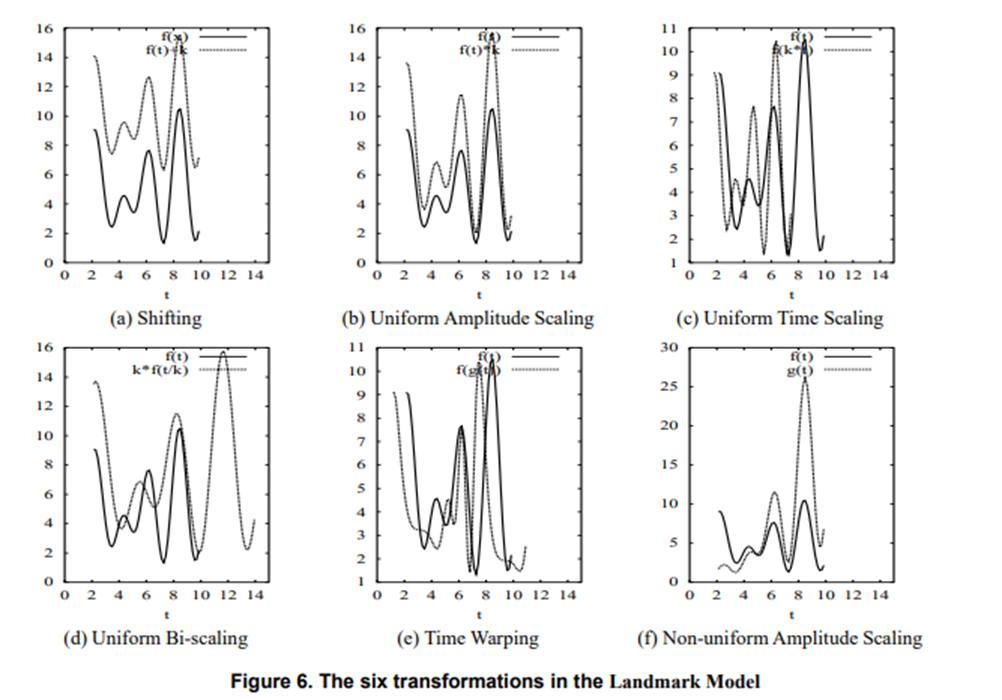
\includegraphics[scale=0.4]{figures/03-teoria/theSixTransformationsInTheLandmarkModel.png}
                \caption{Transformations in Landmark Model}
                \label{fig:scr46}
            \end{figure}
            \par
            Wybór cech charakterystycznych:
            Różne cechy są wykorzystywane do różnych zastosowań, od prostych cech (minima lokalne, maksima lokalne, punkty przełamania) do bardziej skomplikowanych
            Im więcej typów cech, tym dokładniejsze wyniki
            Punkt charakterystyczny n-tego rzędu danej krzywej jest wtedy, gdy pochodna n-tego rzędu znajduje się na tym punkcie – lokalne minima/maksima są punktami 1 rzędu, a punkty przegięcia – 2 rzędu
            Im bardziej zmienny wykres, tym mniejsze znaczenie mają punkty charakterystyczne wyższych rzędów
            \par
            Wygładzanie: Minimal Distance/Percentage Principle (MDPP) 
            Przykład MDPP(5, 5\%) – znaczy: pomiar raz na 5 dni, od 5\% wzrost lub spadek zaczyna być znaczący. Zmiany większe niż 5\% nie zostaną wygładzone
            \par 
            Obliczanie podobieństwa: Porównujemy sekwencje landmarków (a nie surowych danych)
            \begin{itemize}
                \item Pomiar niezgodności (dissimilarity measurement)
                \item Pomiar zgodności (z wykorzystaniem MDPP)
            \end{itemize}
        
        \subsection{Dynamic Time Warping}
        \label{theory:DTW}
            Metoda zakłada znalezienie optymalnego dopasowania punktów jednego przebiegu do drugiego, który ma najmniejszy koszt i spełnia wszystkie z poniższych warunków:
            Założenia przy porównywaniu dwóch sekwencji:
            \begin{itemize}
                \item Pierwsze oraz ostatnie punkty przebiegów są dopasowane do siebie
                \item Przebieg nie cofa się w czasie podczas dopasowywania
                \item Podczas dopasowania nie można wykonać zbyt długich kroków
                \item Koszt dopasowania jest sumą lokalnych odległości na tej ścieżce
            \end{itemize}
            Charakterystyka algorytmu:
            \begin{itemize}
                \item Radzi sobie ze skalowaniem czasu 
                \item Radzi sobie z przesunięciem czasu
                \item Bardziej zwraca uwagę na konkretne wartości, w porównaniu do Landmark Similarity, który głównie zwraca uwagę na punkty zwrotne
            \end{itemize}
        
        \subsection{Longest Common Subsequence}
            Jeżeli S1 i S2 to dwa ciągi, to Z jest ich wspólnym podciągiem jeżeli jest podciągiem zarówno S1, jak i S2
            Dwa ciągi są podobne jeżeli:
            (2 * Długość Z )/(Długość S1 + Długość S2) $>$= wybrana wartość progowa 
    
        \subsection{Odległość Euklidesowa}
        \label{theory:Euklides}
             Długość odcinka między punktami
            \begin{itemize}
                \item Podatny na wartości odstające
                \item Nie radzi sobie ze zeskalowanymi wykresami
                \item Wykresy muszą być tej samej długości
                \item TODO:poszukać wariacje odległości Euklidesowej
            \end{itemize}
    \section{Klasyfikacja szeregów czasowych}
        Klasyfikacja to jeden z znanych problemów, które staramy rozwiązywać się przy pomocy uczenia maszynowego. Jej celem jest przypisanie rekordów zbioru danych do odpowiedniej grupy. Klasyfikacja używa odpowiedniej funkcji mapującej zbiór cech na klasę, gdzie funkcja ta nauczona jest na zbiorze danych treningowych\cite{Classification_theory}. Przykładowe algorytmy, które rozwiązują ten problem to \textit{Support Vector Machine (SVM)}, \textit{Drzewa decyzyjne}, \textit{KNN} i wiele innych, jednak niekonieczne nadają się one do problemu szeregów czasowych.
        
        W przypadku szeregów czasowych nie mamy do czynienia z zbiorem cech dla obserwacji, lecz z pomiarami zebranymi w jakimś okresie czasu. Przykładowo pomiar temperatury w ciągu dnia. Do klasyfikacje trzeba brać pod uwagę szereg jako całość a nie pojedyncze obserwacje. Dodatkowo dany szereg może posiadać więcej niż jeden typ obserwacji, wtedy poza temperaturą, mierzymy przykładowo wilgotność i prędkość wiatru. Innym czynnikiem wpływającym na zdatność algorytmu do klasyfikacji szeregów czasowych jest jego zdolność do radzenia sobie z obserwacjami o różnej długości. Jeżeli badamy pogodę każdego dnia to szeregi będą równe (24 godziny), ale nie zawsze tak jest. Badane zjawisko może mieć nieregularną długość i wtedy każda obserwacja może mieć różną długość trwania (przykładowo zużycie zasobów podczas działania algorytmu). Biorąc pod uwage te wszystkie cechy szeregów czasowych szukaliśmy specyficznych algorytmów, które poradzą sobie z tymi wyzwaniami.
        
        \subsection{ROCKET}
            ROCKET, czyli \textbf{R}and\textbf{O}m \textbf{C}onvolutional \textbf{KE}rnel \textbf{T}ransform wykorzystuje, jak nazwa wskazuje, losowe kernele konwolucyjne do transformacji szeregów czasowych, w celu użycia wyniku tej operacji jako cech w klasyfikatorze \cite{Rocket_classifier}. Autorzy wspierali się tym, że wykorzystanie neuronowych sieci konwolucyjnych jest efektywne dla szeregów czasowych. Podali argumenty za tym, że wykorzystanie losowych kerneli konwolucyjnych oraz wykorzystanie ich wyjściowych transformacji jako cechy wejściowe dla innego klasyfikatora jest wykorzystywane w innych przypadkach z sukcesem. 
            
            Metoda ta wykorzystuje ekstremalną ilość kerneli (domyślnie używali 10.000), w których każdy generuje 2 wartości, w ten sposób każdy szereg czasowy ma wytworzoną dużą ilość cech (w przypadku domyślnych ustawień 20.000 cech). Autorzy twierdzą, że im więcej jąder tym większa dokładność klasyfikacji kosztem czasu przetwarzania. Algorytm klasyfikacji użyty po transformacjach może być dowolny, jednak autorzy polecają klasyfikatory liniowe (domyślnie użyta została \textit{regresja grzbietowa} (ang. Ridge Regression)).
            
            Główną zaletą tego podejścia poza dokładnością, która jest na równi (jak nie lepsza) z innymi nowoczesnymi metodami klasyfikacji szeregów czasowych, jest czas przetwarzania. Złożoność tego algorytmu zależy głównie od liczby kerneli, a poza tym od liczby przykładów oraz długości przebiegów czasowych. Drugim czynnikiem wpływającym na czas potrzebny na wykonanie obliczeń jest złożoność użytego klasyfikatora, więc w przypadku regresji grzbietowej zależy ona od wielkości zbioru i liczby badanych cech. Poprzez eksperymenty w pracy, autorzy pokazali, że w porównaniu z innymi algorytmami czas trwania klasyfikacji jest niższy od reszty dla tej samej liczby przykładów z utrzymaniem podobnej dokładności, co może być dobrą cechą dla naszych przyszłych eksperymentów.
            
            Podsumowując tą sekcje, metoda ROCKET zdaję się być dobrym do sprawdzenia w naszej pracy. Autorzy tekstu pisali, że implementacja w ramach której wykonywali eksperymenty była wykonana w języku Python, więc powinna być możliwość wykorzystania jej w naszych eksperymentach. Jedyne czego brakowało w artykule to wykorzystanie algorytmu dla wielowymiarowych szeregów czasowych, jednak w podsumowaniu napisali, że jest to następny krok w badań. Z względu na to jest szansa, że ten algorytm został przystosowany dla takich zbiorów danych.
        \subsection{HIVECOTE2}
            HIVECOTE, czyli Hierarchical Vote Collective of Transformation-based Ensembles to heterogeniczny meta zbiór metod klasyfikacji szeregów czasowych \cite{HiveCote}. Każdy z zawartych algorytmów dotyczy innej domeny. Można w tej metodzie znaleźć takie algorytmy jak \textit{shapelets}, słownikach bazujących na modelu ""bag-of-words"" oraz metody interwałowe. Zgodnie z badaniami autorów pracy, HIVECOTE2 średnio jest jednym z najlepszych klasyfikatorów szeregów czasowych.
            
            Konkretne modele zawarte w ramach drugiej wersji tego algorytmu to: 
            \begin{itemize}
                \item \textit{Shapelet Transform Classifier}
                \item Dostosowana wersja wcześniej wspomnianego algorytmu \textit{ROCKET} nazwana \textit{ARSENAL}
                \item \textit{Temporal Dictionary Ensemble (TDE)}
                \item \textit{Diverse Representation Canonical Interval Forest (DrCIF)}
            \end{itemize}
            Każdy z tych algorytmów jest uczony osobno i dodatkowo na potrzeby ostatecznego wyniki musi zwrócić estymacje swojej dokładności (ang. accuracy) na nieznanych im wcześniej danych. Podczas predykcji, każda z metod zwraca prawdopodobieństwo przynależności badanego szeregu do danej klasy po czym obliczana jest średnia ważona. Wagi to wcześniej obliczona dokładność poszczególnych algorytmów, która jest zmniejszona poprzez potęgowanie przez jakąś wartość (domyślnie jest to 4). Poniższy rysunek \ref{fig:hive_example} pokazuje przykładowe działanie tego algorytmu w praktyce dla problemu trzy-klasowego:
            
           \begin{figure}[H]
                \centering
                \captionsetup{justification=centering,margin=0.5cm}
                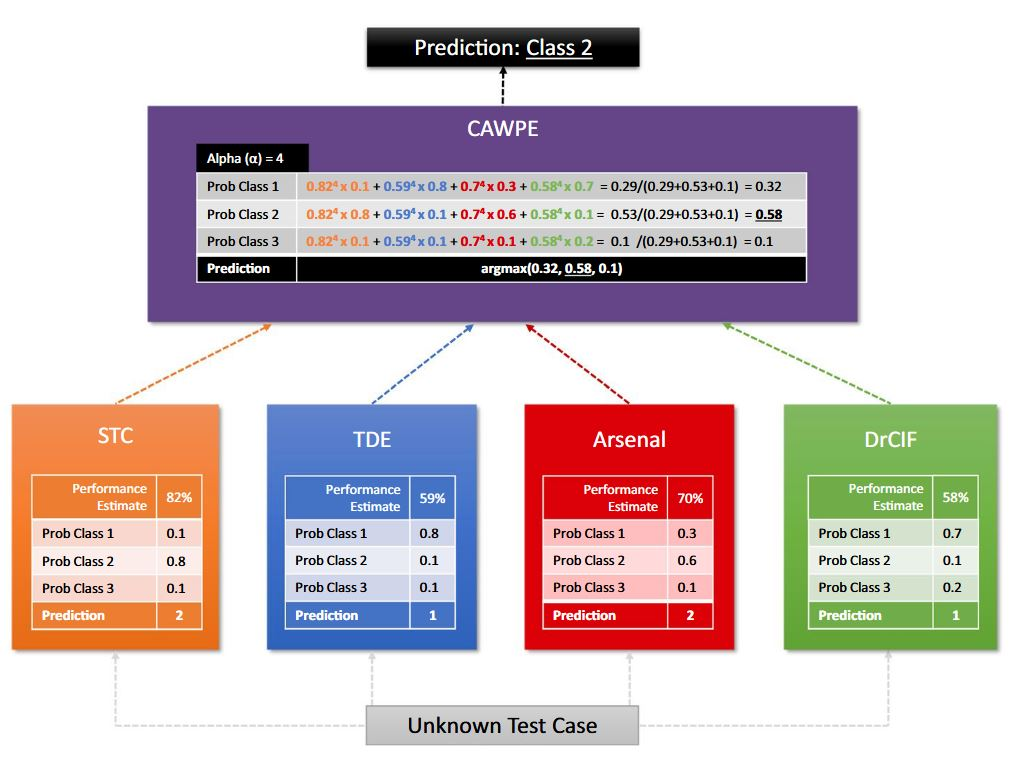
\includegraphics[scale=0.6]{figures/03-teoria/HIVE.JPG}
                \caption{Przykładowe działanie algorytmu HIVECOTE2 \cite{HiveCote}}
                \label{fig:hive_example}
            \end{figure}
            
            Jednym z zarzutów dla metody HIVECOTE2 jest jego długi czas uczenia. W porównaniu z algorytmem ROCKET jest on rzeczywiście powolny. W pracy autorzy zmieścili porównanie, gdzie ROCKET wykonuje się ponad 100 razy szybciej od algorytmu HIVECOTE2. Jednak twórcy umożliwiają ograniczenie czasu procesowania co może pozwolić nam na wygodne wykorzystanie tej metody do badań, kosztem dokładności obliczeń.
            
            Podsumowując, ten algorytm jest warty uwagi jeżeli znajdziemy jego implementacje w języku Python. Zgodnie z badaniami z opisywanej w tej sekcji pracy jest to algorytm, który powinien mieć bardzo dokładne wyniki, jeżeli pozwolimy mu wykonywać się bez ograniczeń czasowych. Jeżeli wyniki będą zadowalające dla wersji ograniczonej czasowo, eksperymenty zapewne wykonamy z tym ograniczeniem w celu oszczędzenia czasu.
        \subsection{KNN-DTW}
            Poza wyspecjalizowanymi podejściami do klasyfikacji szeregów czasowych, warto sprawdzić czy bardziej ogólne metody nadają się do badania tego problemu. Jednym z takich algorytmów jest KNN albo K-najbliższych sąsiadów (ang. K-nearest neighbor). Ta metoda przechowuje wszystkie dostępne rekordy i nadaje klasę nowemu przypadkowi na podstawie zmierzonego podobieństwa. K jest to liczba sąsiadów, których "głos"  jest wzięty pod uwagę do predykcji. Przykładowo jeżeli k = 3 to koło dookoła nowego rekordu, gdzie promieniem jest podobieństwo, będzie zawierało w sobie 3 inne przykłady. Te przykłady są wzięte do głosowania aby określić przynależność do klasy badanego przykładu \cite{Classification_theory}. 
            
            Używając tego algorytmu do przebiegów czasowych, należy wybrać odpowiednią miarę podobieństwa pasującą do tego problemu. W poprzedniej sekcji \ref{theory:podobienstwo} zbadaliśmy znane podejścia i najbardziej wyróżniającą się miarą jest \textit{Dynamic Time Warping}. Użycie tego podejścia w połączeniu z algorytmem K-NN jest sprawdzoną metodą i udowodniono, że jakość klasyfikacji w tym przypadku jest bardzo dobra, osiągająca ok. 80\% dokładności \cite{KNNDTW}. Autorzy pracy również wzięli pod uwagę inne miary podobieństwa, jednak w przypadku klasyfikacji DTW osiągnął najlepsze wyniki. Wiemy też, że istnieją implementacje tego algorytmu w języku Python co daje nam możliwość użycia go w naszej pracy.
    
    \section{Metody normalizacji danych}
        \label{section:norm}
        W pracach zajmujących się uczeniem maszynowym bardzo często występuje normalizacja danych. Przykładowo \cite{RuntimeEstimationALICE} wykorzystuje normalizacje Z-score, a w pracy \cite{BigDataParallelism} twórcy użyli skalowania Min-Max. Wykonuję się ją na etapie przygotowywania danych (ang. Preprocessing) najczęściej w celu poprawienia wyników algorytmów lub czasem nawet algorytmy wymagają znormalizowanych danych dla poprawnego działania \cite{standarization_effects}. Dzięki temu procesowi otrzymujemy wartości, które w zbiorze danych będą miały podobną skale. W tej sekcji opisane zostaną popularne metody normalizacji danych, czyli \textbf{Min-Max} oraz \textbf{Z-score}. Jedna z tych metod zostanie użyta na danych wykorzystywanych w tej pracy.
        
        \subsection{Min-Max}
            Technika normalizacji Min-Max polega na odjęciu od wartości najmniejszej wartości z dziedziny i następnie podzielenie jej przez największą wartość z tej samej dziedziny. Tą metodę można przedstawić za pomocą następującego wzoru: 
            \begin{equation}
            \label{eqn:minmax}
            A'_i = \frac{A_i-min(A)}{max(A) - min(A)}
            \end{equation}
            W ten sposób uzyskujemy przeskalowane wartości z zakresu od 0 do 1. Jest to dobra technika, jeżeli nie znamy rozkładu wartości naszych danych lub jeżeli wiemy, że nie jest to rozkład standardowy.
        
        \subsection{Z-score}
            Ten sposób normalizacji to skalowanie poprzez odjęcie od wartości średniej wszystkich wartości i następnie podzielenia przez odchylenie standardowe zbioru. Wzór prezentuje się następująco:
            \begin{equation}
            \label{eqn:minmax}
            A'_i = \frac{A_i-mean(A)}{std(A)}
            \end{equation}
            Ta technika nie jest ograniczona przez żaden predefiniowany zakres wartości. Sprawia ona że średnia jest równa 0, a odchylenie standardowe 1. Użycie tej metody jest preferowane, jeżeli znamy rozkład wartości i jest on rozkładem standardowym.
